\documentclass[report,openany]{memoir}
\chapterstyle{ell}
\pagenumbering{arabic}


\setlrmarginsandblock{3cm}{*}{*}
\checkandfixthelayout

\usepackage{fourier}
\usepackage{verbatim}
\usepackage{graphicx}
\usepackage{amsmath} 
\usepackage{extarrows}
\usepackage{listings}
\usepackage{url}

\usepackage{colortbl,array}
\usepackage{tabularx}
\newcolumntype{R}{>{\raggedleft\arraybackslash}X}

%\usepackage{trackchanges}
%\addeditor{SH}

\newcommand*{\TitleFont}{%
      \usefont{\encodingdefault}{\rmdefault}{b}{n}%
      \fontsize{16}{20}%
      \selectfont}



%\renewcommand{\maketitlehooka}{Test}
%\renewcommand{\maketitlehookc}{\vspace{3.0cm}\hspace{2.7cm}\vspace{2.2cm}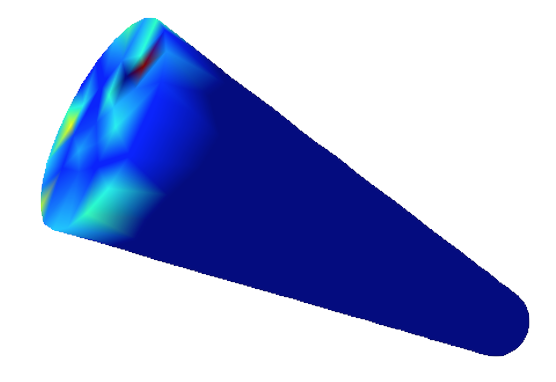
\includegraphics[scale=1.0]{imgs/stochssoutput.png}}

\renewcommand{\maketitlehooka}{
\vspace{-150pt}

\begin{figure}[!hbt]
\hspace{-70pt}

\includegraphics[width=40pt,height=40pt]{ucsbseal.png}

\includegraphics[width=40pt,height=40pt]{uulogo.png}
\vspace{150pt}
\end{figure}
}

\title{\rightline{\HUGE StochSS: Stochastic Simulation Service}}
\date{}
\renewcommand{\maketitlehookb}{\vspace{-0.4cm}{\rightline{\LARGE User Guide and Tutorial}}\vspace{11.3cm}}

\renewcommand{\maketitlehookc}{\hspace{10.2cm}
\includegraphics[scale=0.7]{imgs/stochsslogo.png}}


\definecolor{warningbackground}{RGB}{255,255,255}

\newcommand{\warning}[1]{
    \hspace{\baselineskip}\hrule
    \begin{tabularx}{\linewidth}{
        >{\columncolor{warningbackground}}c
        >{\columncolor{warningbackground}}X}
        \raisebox{\dimexpr2\baselineskip-\height}
        {
\includegraphics[scale=0.3]{imgs/warningsymbol.png}}&
        \raisebox{\tabcolsep}{\strut}#1\raisebox{-\tabcolsep}{\strut}
    \end{tabularx}
    \hrule\vspace{\baselineskip}
}

\newcommand{\tip}[1]{
    \hspace{\baselineskip}\hrule
    \begin{tabularx}{\linewidth}{
        >{\columncolor{warningbackground}}c
        >{\columncolor{warningbackground}}X}
        \raisebox{\dimexpr2\baselineskip-\height}
        {
\includegraphics[scale=0.3]{imgs/tipsymbol.png}}&
        \raisebox{\tabcolsep}{\strut}#1\raisebox{-\tabcolsep}{\strut}
    \end{tabularx}
    \hrule\vspace{\baselineskip}
}


\usepackage{xcolor}
\usepackage[many]{tcolorbox}
\tcbuselibrary{listings}

\definecolor{light-gray}{gray}{0.95}

% the space reserved between for the ``In'' numbers and the code
\newlength\inwd
\setlength\inwd{1.3cm}

\newcounter{ipythcntr}

\newtcblisting{ipythonnb}[1][\theipythcntr]{
  enlarge left by=\inwd,
  width=\linewidth-\inwd,
  enhanced,
  boxrule=0.4pt,
  colback=light-gray,
  listing only,
  top=0pt,
  bottom=0pt,
  overlay={
    \node[
      anchor=north east,
      text width=\inwd,
      font=\footnotesize\ttfamily\color{blue!50!black},
      inner ysep=2mm,
      inner xsep=0pt,
      outer sep=0pt
      ] 
      at (frame.north west)
      {\stepcounter{ipythcntr}In [#1]:};
  }
  listing options={
    basicstyle=\footnotesize\ttfamily,
    language=python,
    escapechar=�,
    showstringspaces=false,
  },
}



\begin{document}
\maketitle

\tableofcontents

%\chapter{Introduction}

%\section{Prerequisites}

\begin{itemize}
\item StochSS 1.4 (or later) installed on your computer (please follow download and installation instructions at \url{www.stochss.org}). 
\item A basic understanding of well-mixed discrete stochastic simulations and models based on ordinary differential equations \cite{dan,sundials}.
\item A basic knowledge of the mesoscopic reaction-diffusion master equation and of the Next Subvolume Method (NSM) \cite{nsm}.
\item  A basic knowledge of the functionalities in the StochSS GUI (please consult the \textit{Basic Introduction to StochSS} tutorial).
\item The following login screen appears in your browser; please log in.
\end{itemize}

\begin{figure}[!ht]
\centering
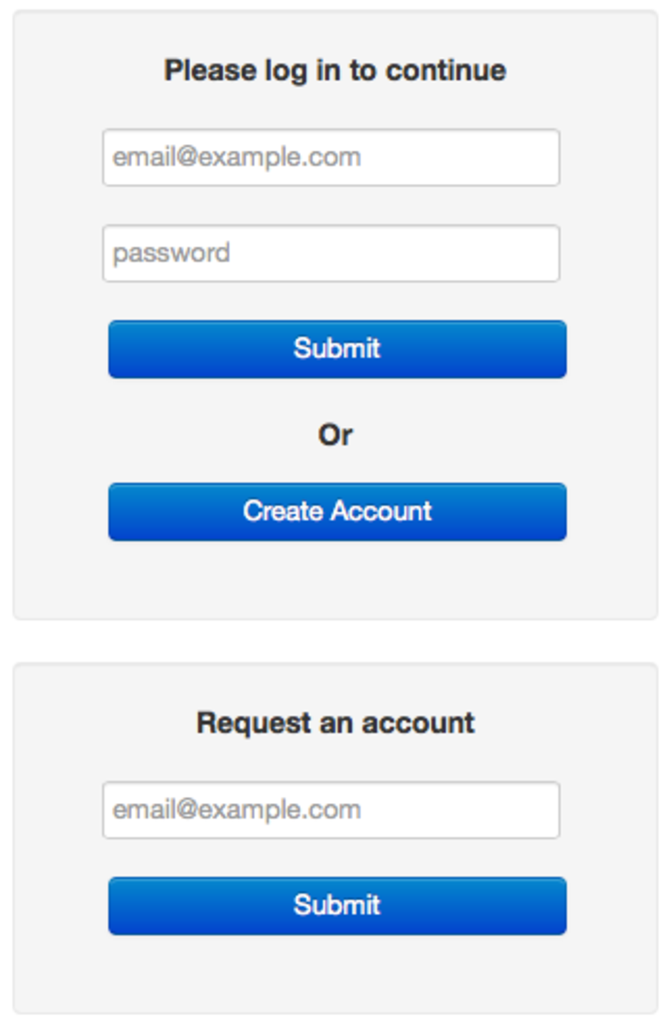
\includegraphics[scale=0.55]{T6/user-login.pdf}
\end{figure}

%!TEX root = main.tex

\chapter{Installation}

StochSS supports Mac OS X, Linux, and Windows through the Docker platform. To install StochSS, you'll need to install Docker on your computer, and then use the appropriate StochSS launch application to initialize and run your StochSS Docker container.

For instructions on how to install the latest version of StochSS for your platform, please see the StochSS website http://www.stochss.org/. The source code, together with installation instructions, is also available on GitHub: https://github.com/StochSS/stochss/tree/master/stochss-launcher.

%
%\section{Mac OS X}
%
%\subsection{Running StochSS}
%\begin{itemize}
%	\item Install Docker Toolbox using directions here: https://docs.docker.com/engine/installation/mac/\#installation
%	\item Download the Mac OS X application zip file: http://stochss.org/releases/stochss.mac.1.7.0.zip
%	\item Double click the icon to launch server.
%\end{itemize}
%Uninstalling StochSS can be performed with the uninstall app included with the zip file above.
%
%
%\subsection{When things go wrong}
%
%Leaving StochSS is running while the computer goes to sleep can cause the network configuration of the virtual machine to change unexpectedly when the computer is woken up again. This means that StochSS could become temporarily inaccessible. Performing the following steps may solve this: Open a Docker Quickstart terminal window and run:
%\begin{itemize}
%	\item \begin{verbatim}docker-machine start stochss1-7\end{verbatim}
%	\item \begin{verbatim}docker-machine ssh stochss1-7\end{verbatim}
%	\item \begin{verbatim}docker stop stochsscontainer1_7\end{verbatim}
%	\item \begin{verbatim}docker start stochsscontainer1_7\end{verbatim}
%	\item exit
%\end{itemize}
%
%Our suspicion is that when we ssh into the virtual machine, it's network configuration is reset/corrected.
%
%
%\section{Linux}
%StochSS requires Docker to run. The StochSS run script (stochss.sh) uses Docker to download and run StochSS inside a Docker container (this is basically a lightweight virtual machine). Docker and this script are all you need to run Stochss on your Linux computer.
%
%Note: The Ubuntu 12.04 default kernel is too old to support Docker. 12.04 users can instead just run StochSS without the container. Download the package at http://stochss.org/releases/stochss.linux.1.7.0.tgz and refer to the old installation instructions at http://www.stochss.org/wordpress/?page\_id=224\#linux.
%
%\subsection{Running StochSS}
%\begin{itemize}
%	\item Install Docker using directions here: https://docs.docker.com/engine/installation/linux/
%	\item Open up a terminal window
%	\item Download the Ubuntu run script : \begin{verbatim}curl -o stochss.linux.1.7.0.tgz http://stochss.org/releases/stochss.linux.1.7.0.tgz\end{verbatim}
%	\item Untar the folder and navigate inside : \begin{verbatim}tar -xzf stochss.linux.1.7.0.tgz; cd stochss.linux.1.7.0\end{verbatim}
%	\item Run the script (the script will ask for your administrative password): \begin{verbatim}./stochss.sh\end{verbatim}
%\end{itemize}
%
%\subsection{Uninstalling StochSS}
%\begin{itemize}
%	\item Open up a terminal window
%	\item Run:
%\begin{itemize}
%	\item \begin{verbatim}sudo docker stop stochsscontainer1_7\end{verbatim}
%	\item \begin{verbatim}sudo docker rm stochsscontainer1_7\end{verbatim}
%\end{itemize}
%\end{itemize}
%
%
%\section{Windows}
%
%StochSS requires Docker Toolbox for Windows to run. This means you will need a 64 bit Windows installation that supports Docker (Windows 64 7, 8, and 10, should all work).
%
%Please note:
%\begin{enumerate}
% 	\item StochSS does not run on Microsoft Edge browser. The recommended browser is Google Chrome.
% 	\item You may have to enable virtualization in the BIOS (Use this Microsoft Virtualization detector to check if virtualization is enabled in your system: https://www.microsoft.com/en-us/download/details.aspx?id=592. If it's not, please enable it from the BIOS first).
%\end{enumerate}
%
%\subsection{Running StochSS}
%
%\begin{enumerate}
% 	\item Install Docker Toolbox using directions here: https://docs.docker.com/engine/installation/windows/
%\begin{itemize}
% 	\item To paste text from your clipboard to Docker Quickstart terminal, \textit{right click} onto the terminal screen.
% 	\item To copy text from the Docker Quickstart terminal onto your clipboard, highlight the desired text and press \textit{enter/return}.
%\end{itemize}
%
% 	\item Open the Docker QuickStart Terminal. Run the following commands:
%\begin{itemize}
% 	\item \begin{verbatim}docker-machine start stochss1-7 || docker-machine create --driver virtualbox stochss1-7\end{verbatim}
% 	\item \begin{verbatim}eval "$(docker-machine env stochss1-7)"\end{verbatim}
%\end{itemize}
%
%This will start/create a Virtual Machine called `stochss1-7', and give you terminal access to it. StochSS will run in this machine. To verify that the machine is running, run the following command:
%\begin{itemize}
% 	\item \begin{verbatim}docker-machine ls\end{verbatim}
%\end{itemize}
%You should see that the status of machine `stochss1-7' is <em>running</em>.
%
%Please note the IP address of the of the machine `stochss1-7'. Run the following command to determine the IP address:
%\begin{itemize}
% 	\item \begin{verbatim}docker-machine ip stochss1-7\end{verbatim}
%\end{itemize}
%
% 	\item If this is the first time you're starting StochSS, run the following to start StochSS container:
%\begin{itemize}
%
%\begingroup
%    \fontsize{8pt}{12pt}\selectfont
% 	\item \begin{verbatim}docker run -i -t -p 8080:8080 -p 8000:8000 --name=stochsscontainer1_7 stochss/stochss-launcher:1.7 "/bin/bash"\end{verbatim}
%\endgroup
%
%\end{itemize}
%This will download the StochSS docker image, create the StochSS docker container and give terminal access to it. \textbf{PLEASE NOTE}: when this is complete you will get the message: \begin{verbatim}bash: /usr/local/share/dolfin/dolfin.conf: No such file or directory\end{verbatim}. �This is not an error, please continue with the installation.
%
%Otherwise, if you already have a StochSS docker container (i.e. when you use StochSS subsequently), run
%\begin{itemize}
% 	\item \begin{verbatim}docker start stochsscontainer1_7\end{verbatim}
% 	\item \begin{verbatim}docker exec -ti stochsscontainer1_7 /bin/bash\end{verbatim}
%\end{itemize}
%
% 	\item Run the following commands to start the server:
%\begin{itemize}
% 	\item \begin{verbatim}cd stochss-master\end{verbatim}
% 	\item \begin{verbatim}./run.ubuntu.sh -a \textbf{the_ip_address_you_noted_in_Step_2_above} -t secretkey\end{verbatim}
%\end{itemize}
%Navigate to the URL displayed to access StochSS.
% 	\item Follow the instructions on the terminal to kill the server process. After that, run the following commands to stop the container:
%\begin{itemize}
% 	\item \begin{verbatim}exit\end{verbatim}
% 	\item \begin{verbatim}docker stop stochsscontainer1_7\end{verbatim}
% 	\item \begin{verbatim}docker-machine stop stochss1-7\end{verbatim}
%\end{itemize}
%These commands will stop the container and virtual machine. The terminal window can now be safely closed.
%\end{enumerate}
%
%\subsection{Uninstalling StochSS}
%
%\begin{enumerate}
% 	\item Open the Docker Quickstart terminal
% 	\item Run the following command:
%\begin{verbatim}docker-machine rm stochss1-7\end{verbatim}
%\end{enumerate}
%
%\subsection{When things go wrong}
%
%\begin{enumerate}
% 	\item Launching and using StochSS on Windows is error-prone. Some useful commands that may help you in figuring out what's going on when things don't work as expected are:
%\begin{itemize}
% 	\item \begin{verbatim}docker-machine ls\end{verbatim} will list the virtual machines running and their status.
% 	\item \begin{verbatim}docker ps\end{verbatim} will list the containers that are \textit{running}.
% 	\item \begin{verbatim}docker ps -aq\end{verbatim} will list all containers in the virtual machine, running or stopped.
%\end{itemize}
%
% 	\item Leaving StochSS is running while the computer goes to sleep can cause the network configuration of the virtual machine to change unexpectedly when the computer is woken up again. This means that StochSS could become temporarily inaccessible. Performing the following steps may solve this:Open a Docker Quickstart terminal window and Run:
%\begin{itemize}
% 	\item \begin{verbatim}docker-machine start stochss1-7\end{verbatim}
% 	\item \begin{verbatim}docker-machine ssh stochss1-7\end{verbatim}
% 	\item \begin{verbatim}docker stop stochsscontainer1_7\end{verbatim}
% 	\item \begin{verbatim}docker start stochsscontainer1_7\end{verbatim}
% 	\item \begin{verbatim}exit\end{verbatim}
%\end{itemize}
%Follow the instructions in this guide to start StochSS.
%
%Our suspicion is that when we ssh into the virtual machine, it's network configuration is reset/corrected.
%\end{enumerate}
%
%\section{Note on security}
%When you run StochSS, it is encapsulated inside a virtual machine. If something goes wrong with the StochSS virtual machine, it is isolated from everything else on your system.



\chapter{Basic Introduction}
\label{chapter1}
This tutorial will guide you through the basic features of StochSS. You will become familiar with the \textbf{Model Editor} and the \textbf{Simulation Manager}. You will learn how to create your own model, which can be population or concentration-based, and how to simulate it using either an ordinary differential equation (ODE) solver or the stochastic simulation algorithm (SSA).

\section{Creating Administrator and Standard User Accounts}
At the end of a successful installation process, your default browser will launch and you will be asked to create an admin account as in Figure \ref{fig:admin} (there is only one admin account for the entire system).
Once the admin account is created you will be forwarded to a regular login page where you can log in to StochSS.

\begin{figure}[!htb]
\centering
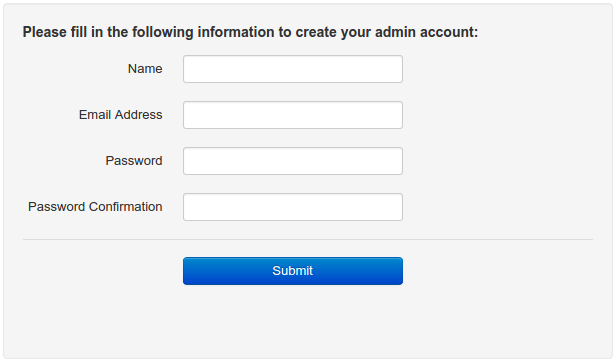
\includegraphics[scale=0.64]{T1/admin.png}
\caption{Administrator login page}
\label{fig:admin}
\end{figure}

Users can click \textbf{Create Account} to request an account.
The account will not be accessible until the admin approves it in the \textbf{Admin Panel} (the admin can also delete active users as well as reset their passwords there).
%
%\begin{figure}[!htb]
%\centering
%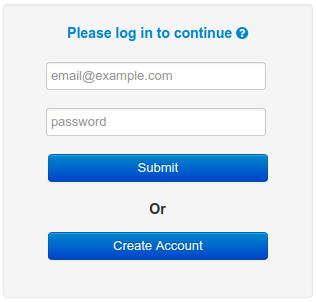
\includegraphics[scale=0.64]{T1/login.png}
%\caption{User login page}
%\label{fig:login}
%\end{figure}

\section{Importing a Model}
The \textbf{Model Editor} will let you create new or modify existing well-mixed stochastic biochemical models as well as deterministic models based on ODEs.
The best way to get started with the model editor is to import an example model and look at the different sections.

\subsection{Importing an existing model}

\underline{Option 1: StochSS Public Library}
\begin{itemize}
  \item Navigate to the \textbf{Model Editor} page.
  \item Click \textbf{Import from Public Library} in the right-hand toolbar.
  \item Select a model from the Public Library and click \textbf{Copy Model to Library}.
\end{itemize}

\noindent\underline{Option 2: Stochkit2 XML}
\begin{itemize}
  \item Navigate to the \textbf{Model Editor} page.
  \item Click \textbf{Import from .XML} in the right-hand toolbar.
  \item Select an XML file. A collection of example models can be found in the \textit{examples} directory within the StochSS install folder.
  \item Click \textbf{Import}.
\end{itemize}

After importing the XML file or public model, StochSS should display the imported model in the model editor.
Look through the page to see how the different \textbf{Species}, \textbf{Parameters}, and \textbf{Reactions} are defined.
By clicking \textbf{Export to .zip} or \textbf{Export to Public Library} the model can be shared across computers or shared amongst users of the same StochSS.

\section{Creating a New Model}
An example population model is defined by the following two reactions:
\begin{equation}
\label{eq:tut1-reac1}
\begin{aligned}
S0 + S0 &\xrightarrow{k1} S1\\
S1 &\xrightarrow{k0} \emptyset .  
\end{aligned}
\end{equation}

To create this model:
\begin{itemize}
  \item Navigate to the \textbf{Model Editor}.
  \item Click \textbf{Add Model} and select \textit{Population, Well-mixed}.
  \item Rename the model to \textit{example}.
  \item Click \textbf{Create Species} twice to create two species.
  \item By default the species are named $S0$ and $S1$. Set the initial condition for $S0$ to $1000$ and the initial condition for $S1$ to $0$.
  \item Similarly to above, click \textbf{Add Parameter} twice to add two parameters.
  \item By default they will be named $k0$ and $k1$. Set $k0$ to $0.0001$ and $k1$ to $0.05$.
  \item Click \textbf{Add Reaction} to add two reactions. Select the reactants, products, rates and reaction types corresponding to \eqref{eq:tut1-reac1}. Compare to Figures \ref{fig:reaction2} and \ref{fig:reaction1} to verify the settings.
\end{itemize}

\begin{figure}[!htb]
\centering
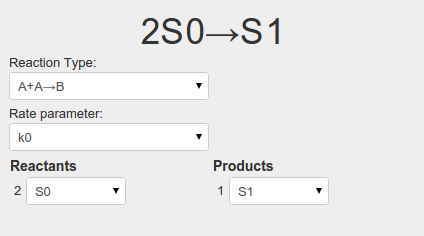
\includegraphics[scale=0.64]{T1/reaction2.png}
\caption{Decay reaction}
\label{fig:reaction2}
\end{figure}

\begin{figure}[!htb]
\centering
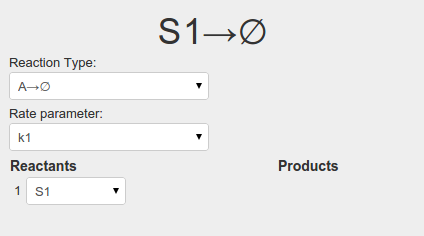
\includegraphics[scale=0.64]{T1/reaction1.png}
\caption{Dimerization reaction}
\label{fig:reaction1}
\end{figure}

\section{Running a Simulation and Visualizing results}

For this section, create or import a model using the directions above.

\begin{itemize}
  \item Navigate to the \textbf{Simulation Manager} page.
  \item Select the model you wish to simulate and click \textbf{Next}.
  \item Setup your simulation parameters: name, time, data storage frequency, realizations and solver type. 
  \begin{itemize}
    \item If you are simulating a population-based model you can choose between the deterministic and the stochastic solvers.
    %\item If you choose the deterministic solver, you have the possibility to perform sensitivity analysis on a set of chosen parameters related to your model.
    \item Concentration-based models can only be simulated using the deterministic solver.
  \end{itemize}  
  \item Click \textbf{Run Locally}. You will be automatically forwarded to the \textbf{Job Status} page.%When the job runs, StochSS should automatically transition to the \textbf{Job Status} page.
  \item Click \textbf{View} to open the \textbf{Job summary} page, where you can visualize the simulation's trajectories.
  \item Click \textbf{Access Local Data} to download a raw copy of the data. This can be used to share data between StochSS installations or perform manual data analysis.
\end{itemize}

\subsection{Converting a concentration model to population}
Create a concentration model or use the directions above to import one. Both Lotka-Volterra examples are concentration based and are available both as XML files and Public Library models.

\begin{itemize}
  \item Select the newly minted concentration model.
  \item Click \textbf{Convert to Population} on the right-hand toolbar to start the conversion process. The model conversion page will open.
  \item To convert a concentration model to a population, a system volume must be specified.
  \item Given a volume, StochSS converts initial conditions through 
  \begin{align}
  \mathrm{initial\_condition\_population} = \mathrm{initial\_condition\_concentration}\times\mathrm{volume}
  \end{align}
   and attempts to convert the reaction rates. It is not always possible to convert reaction rates automatically. If automatic conversion fails the conversion still proceeds, but the user now has to correct the reactions that were not automatically converted.
  \item Click \textbf{Finish conversion} at the bottom left of the page to create a population-based model. This newly created population model can be simulated using both deterministic and stochastic solvers.
  \item Click \textbf{Cancel conversion} to cancel the conversion.
\end{itemize}

\warning{The conversion process operates correctly only if the model to be converted is entirely based on the mass action kinetics allowed in Gillespie Stochastic Simulation Algorithm \cite{dan}. If the model to be converted is not entirely based on mass action kinetics, the conversion tool only converts what it can. }

\section{Backup and Transfer your Data}
You can backup or share your saved models and simulations with the StochSS ZIP format. There are three ways to create StochSS ZIP files:

\begin{itemize}
\item Navigate to the \textbf{Backup} page in the left-hand toolbar and click \textbf{Export}. This exports a ZIP containing all models and simulation results for the current user. There is an option to export all data for all users if this page is accessed with the admin account.
\item Select a model on the \textbf{Model Editor} page and click \textbf{Export to .zip}.
\item Click \textbf{View} on the \textbf{Job Status} page, and then click \textbf{Access local data}.
\end{itemize}

These ZIP files can all be imported into StochSS on the \textbf{Backup} page. To import the contents of a ZIP file into StochSS:

\begin{itemize}
\item Navigate to the \textbf{Backup} page.
\item Click \textbf{Import}.
\item Select the ZIP file to upload. The file should automatically begin uploading, and then appear in a table of ZIP archives below.
\item Select the ZIP file in the table.
\item Define the behavior of the import by either limiting what files get imported or specifying how overlapping names are handled.
\item Click \textbf{Import} at the bottom of the page.
\end{itemize}

\subsection{Exporting data from an old version of StochSS (1.2 or previous)}
To create a backup archive from an older version of StochSS, execute the following command from a terminal window in the directory of your new StochSS installation:
\begin{verbatim}
./exportserver.py path_to_your_old_StochSS_installation
\end{verbatim}
You can import the backup archive you created as described above.


\chapter{Sensitivity Analysis}

StochSS implements forward sensitivity analysis based on the CVODES ODE solver \cite{sundials}.

For instance, if we consider the population of $P$ and the parameter $Vmax$ in the Michaelis-Menten model in the \textbf{Public Library}. The sensitivity of the rate of the increase in population $P$ to the parameter $Vmax$ is defined as the incremental rate of change in $P$ due to incremental changes in $Vmax$:

\begin{equation}
\frac{\partial P(t)}{\partial V_{max}}.
\end{equation}

These are the sensitivities that StochSS produces. There is no rescaling to make these sensitivities unitless.

\section{Example: Michaelis-Menten}

In this example we will study the Michaelis-Menten model from the StochSS Public Library. Details on the model can be found in \cite{wiki-michaelis-menten}.
\begin{itemize}
\item Import the model from the public library. By default, it will be called \textit{michaelis\_menten}.
\item Navigate to the \textbf{Simulation Manager}, select the model, and click \textbf{Next}.
\item Under \textbf{Simulation type}, select \textit{Deterministic + Sensitivity}.
\item You can now select the parameters for which you wish to compute sensitivities. For instance you could select $Km$, $k3$, $mu$, and $Vmax$, to perform sensitivity analysis with only these parameters.
\item Click \textbf{Run Locally}. 
\item Navigate to the \textbf{Job Summary} page to analyze the output. You can plot species trajectories as well as sensitivities.
\end{itemize}


\chapter{StochOptim: Parameter Estimation}
\label{chapter-stochoptim}

StochSS implements parameter estimation for stochastic biochemical systems, StochOptim, via the Monte Carlo expectation-maximization with Modified Cross-Entropy method (MCEM$^2$) \cite{bernie}.
MCEM$^2$ computes maximum likelihood parameter estimates (MLEs) and associated uncertainties in three consecutive phases: cross-entropy, Monte Carlo expectation-maximization (MCEM), and uncertainty quantification \cite{bernie}.

\section{Example: Estimate parameters of a birth-death model}
We consider the Birth-Death model that can be imported from the StochSS Public Library (see Section~\ref{chapter1} for instructions on how to import models in StochSS).
After the model has been imported:
\begin{itemize}
\item Select \textbf{Parameter estimation} from the menu on the left of the screen.
\item Select the model and click \textbf{Next}. This will open the \textbf{Simulation page}.
\item On the Simulation page, select only parameter $k1$. In this example the value of $k2$ is already optimized. This is to make the convergence process faster.
\item Example files (StochOptim input data) for the initial conditions and the trajectories are provided in the \textit{examples} folder (included in your StochSS package) and are named \textit{birthDeathInitial.txt} and \textit{birthDeathTrajectories.txt}, respectively.
\item Click \textbf{Run Locally} to start the parameter estimation.
\item Select \textbf{Job Status} from the menu on the left of the screen to monitor the status of your submitted job. For the example trajectory data, $k1 = 1.0$ and $k2 = 0.03$ are the correct parameter values, so the simulation should converge to somewhere near.
Click \textbf{View Progress} to access the \textbf{Job Summary} page and to view more details about the status of your job. Parameter estimation calculations using MCEM$^2$ are typically time consuming computations. For this simple example, the parameter estimation process took a little less than $20$ minutes on a desktop Intel i7 computer. A more realistic job will take much longer to run.

\item When the job has finished, you can generate a new model using the final estimates of the MCEM$^2$ calculation as follows: scroll to the bottom of the \textbf{Job Summary} page and click \textbf{Create Model from Current Estimates}. 
\item If the job doesn't complete in a reasonable amount of time the job can be stopped manually on the \textbf{Job Status} page, and the parameters can be extracted by clicking \textbf{Create Model from Current Estimates}.
\end{itemize}

\subsection{StochOptim input file format}
The StochOptim input data format consists of two tab-separated text files.
The first file represents the initial conditions of the system, and the second file represents trajectories of it.
Each file has three base columns: \textit{Time}, \textit{Rep}, and \textit{Weight}. Additional columns are added for every species in the model that parameter estimation is to be run on. The \textit{Time} column contains the time values of the various trajectories (and should be set to zero for the initial conditions file). The \textit{Rep} column is used to include multiple trajectories in one file for fitting. Basically each trajectory should have a different \textit{Rep} number. An example of this can be seen by comparing the files \textit{birthDeathTrajectories.txt} and \textit{birthDeathTrajectoriesMulti.txt} in the \textit{examples} folder included in the StochSS package. The \textit{Weight} column is currently unused and should be set to $1$. The rest of the columns should be named after the species (case-sensitive) in the model the data will be fit against, and the columns themselves should contain integers representing the population counts at the various time points.


\chapter{Spatial Stochastic Simulations}


The spatial stochastic simulation capabilities in StochSS are based on PyURDME \cite{urdme}. PyURDME is a general software framework for modeling and simulation of stochastic reaction-diffusion processes on unstructured, tetrahedral (3D) and triangular (2D) meshes. The current core simulation algorithm is based on the mesoscopic reaction-diffusion master equation (RDME) model. The default solver is an efficient implementation of the next subvolume method (NSM) \cite{nsm}.

\section{Example: Annihilation of two species in a cylinder}
We will build a simple annihilation model based on an cylinder geometry. At each end of the cylinder, different chemicals will be produced. When they diffuse and meet at the center, they will annihilate each other.
\begin{enumerate}
\item Navigate to the main \textbf{Model editor}.
\item Add a new model. Select \textit{Population, spatial} in the dropdown menu.
 \item Click \textbf{Mesh} and select \textit{Cylinder}. The cylindrical mesh is divided into three subdomains which can be visualized with the controls below the wireframe view.
\item Add two species, $A$ and $B$, both with diffusion constant 1.
\item Click \textbf{Initial Condition}, select \textit{scatter}, and add 500 molecules of species $A$ in subdomain 1 and 500 molecules of species $B$ in subdomain 3. 
\item Add two parameters, $k0$ and $k1$, and set their values to 1 and 100, respectively.
\item Add three reactions:
\begin{align*}
\textrm{R1}:&\quad \emptyset\overset{k_1}{\rightarrow} A\\
\textrm{R2}:&\quad \emptyset\overset{k_1}{\rightarrow} B\\
\textrm{R3}:&\quad A+B\overset{k_0}{\rightarrow}\emptyset
\end{align*}
\item Reaction $R1$ should be restricted to subdomain 1 and reaction $R2$ to subdomain 3. Reaction $R3$ should be allowed throughout the whole domain.
\item The model is now complete and ready to be simulated.
\item Navigate to the \textbf{Simulation manager} page.
\item Select the spatial model you just created and click \textbf{Next}.
\item Setup the simulation parameters: name, time, data storage frequency, and number of realizations. 
\item You can specify a random seed for the random number generator under \textbf{Advanced Settings}.
\item Click \textbf{Run locally}.
\item In a few seconds you will be directed to the \textbf{Job Status} page where you can check the status of your simulation.
\item Once your simulation is complete, click \textbf{View results} to open the \textbf{Job summary} page, where you can visualize the diffusion of the two species over time within the cylindrical container and download the output files of the simulation.

\end{enumerate}

\section{Visualization (of Annhihilation of two species in a cylinder)}
Full three dimensional spatial stochastic simulations can be difficult to analyze. To simplify the process, StochSS has built in three different methods for visualization of spatial models.

\subsection{Surface Renderings with Domain Clipping}

By default, spatial stochastic simulations are rendered as shown in Figure \ref{surface}. These are surface renderings, but the simulations are volumetric. To see inside the volume, StochSS allows slicing the mesh in half along one axis with a plane and only rendering one of the resultant halves. This is shown in Figure \ref{clipx}

\begin{figure}[!ht]
  \centering
    \includegraphics[width=0.5\textwidth]{surface}
  \caption{ Surface rendering of cylindrical domain. The actual stochastic simulation is run on the dual of the shown mesh, so the color at each node corresponds to the concentration in the corresponding voxel of the dual mesh. Colors are interpolated linearly between nodes. The color scale is not shown for brevity. }
  \label{surface}
\end{figure}

\begin{figure}[!ht]
  \centering
    \includegraphics[width=0.5\textwidth]{clipx}
  \caption{ Surface rendering of cylindrical domain clipping along the X dimension. It is now possible to see concentrations of voxels inside the cylinder. }
  \label{clipx}
\end{figure}

\subsection{Colorized Wireframe Meshes}

The second rendering type is similar to the first, but instead of rendering surfaces only edges are rendered (see Figure \ref{wireframe}). The colorization is the same, it is just ideally easier to see inside the mesh. Similarly to the surface rendering the wireframe renderings can be clipped to get a clearer view of what is happening inside the volume. See Figure \ref{clipy} for a demonstration of clipping a mesh in the Y dimension.

\begin{figure}[!ht]
  \centering
    \includegraphics[width=0.5\textwidth]{wireframe}
  \caption{ Wireframe rendering of cylindrical domain. The colors are handled similarly to in Figure \ref{surface}. }
  \label{wireframe}
\end{figure}

\begin{figure}[!ht]
  \centering
    \includegraphics[width=0.5\textwidth]{clipy}
  \caption{ Wireframe rendering of cylindrical domain clipped in the Y direction. }
  \label{clipy}
\end{figure}

\subsection{Volume Rendering}

The final rendering StochSS offers is a volume rendering (Figure \ref{volume}). It uses a basic ray-tracing implementation that follows the techniques in a paper by Congote \cite{Congote:2011}.

\begin{figure}[!ht]
  \centering
    \includegraphics[width=0.5\textwidth]{volume}
  \caption{ This is the volume rendering of the same data shown above. The idea behind volume rendering is to color darkly areas with high concentrations and leave volumes with low concentrations transparent. The transparency makes it possible to see inside a volume rendering, and so the slicing as shown in the surface and wireframe renderings is not used. }
  \label{ volume }
\end{figure}

\chapter{Cloud Computing}
\label{sec:cc}
\section{Credentials}
StochSS provides the options to run jobs using the Amazon cloud infrastructures. In order to use Amazon Elastic Computing Cloud (EC2), Simple Storage Service (S3) and DynamoDB database, which are all required for running jobs in the cloud, you need an Amazon Web Services (AWS) account and a credential pair (consisting of a secret key and an access key) in hand. 

More information regarding how to create an AWS account and get credentials can be found here: \url{http://aws.amazon.com}

\subsection{Setting Credentials in StochSS}
You must set your credentials in StochSS manually (Figure \ref{fig:1}). Once StochSS validates these, you will be able to launch compute nodes and run jobs in the Amazon cloud.

\begin{figure}[!ht]
\centering
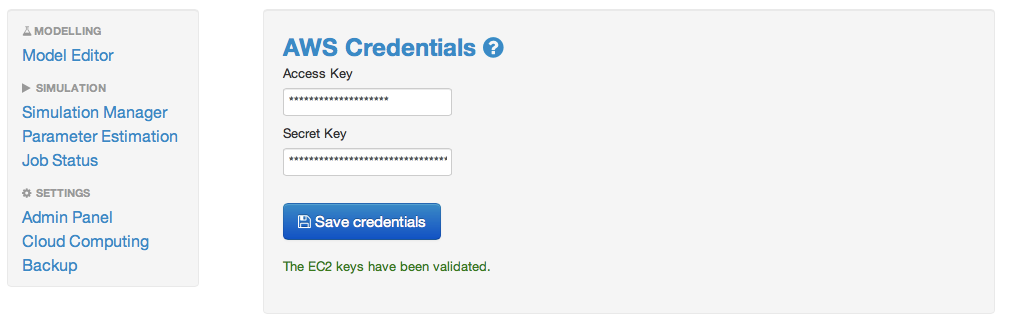
\includegraphics[scale=0.45]{T6/T6_fig_credentials.png}
\caption{Cloud Computing page - Credentials section}
\label{fig:1}
\end{figure}

\begin{enumerate}
\item Navigate to the main \textbf{Cloud Computing} page.
\item Copy your access key to the \textbf{Access Key} text box.
\item Copy your secret key to the \textbf{Secret Key} text box. 
\item Click \textbf{Save credentials} to validate and save your credentials.
\end{enumerate}

\subsection{Launching and Shutting Down Nodes}
Once valid credentials are entered, clicking \textbf{Launch nodes} (Figure \ref{fig:2}) by default will launch one c3.large Amazon instance. This first node is designated the \textbf{head node}. Any other nodes launched are called \textbf{worker nodes}. There can be zero or more worker nodes, and they are c3.larges instance types by default. For information on Amazon instance types, look here: \url{http://aws.amazon.com/ec2/instance-types/}. The head node must be a c3.large or c3.xlarge. The worker nodes can be any combination of t1.micro, m1.small, m3.medium, m3.large, c3.large, and c3.xlarge nodes (chosen in the \textbf{Advanced settings} menu).

Only one head node is needed to run jobs in the cloud. It is possible to access cloud data even when no head nodes are launched. Compute resources and storage resources are billed separately by Amazon. More details can be found at: \url{http://aws.amazon.com/ec2/pricing/}.

\begin{figure}[!ht]
\centering
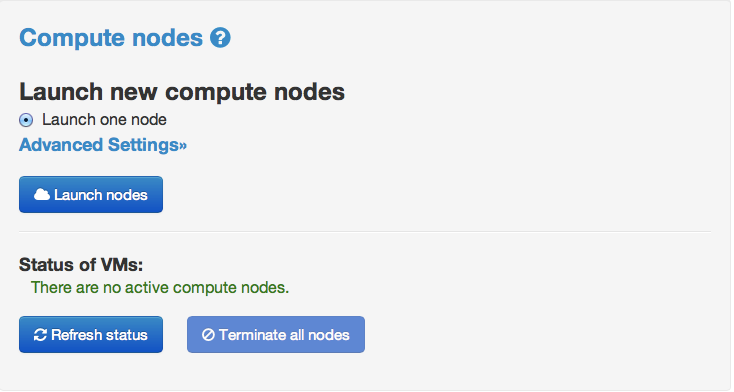
\includegraphics[scale=0.45]{T6/T6_fig_computenode1.png}
\caption{Cloud Computing page - Compute nodes default setting section}
\label{fig:2}
\end{figure}

Launching a node takes time. The \textbf{Refresh status} button can be used to check the launch progress. The \textbf{Terminate all nodes} button terminates all the nodes that StochSS started.

\section{Job Reproduction}
StochSS provides the flexibility to store simulation output in the cloud or delete it and regenerate it later. If simulations are fast but produce large amounts of data, reproducing data only when it is needed can save money.

\subsection{An Example on Job Reproduction}
Reproducing a cloud job is simple:

\begin{enumerate}
\item Launch a compute node.
\item Run a well-mixed or spatial model (everything except parameter estimation jobs can be reproduced).
\item Navigate to the \textbf{Job Status} page.
\item Click \textbf{view} beside the job you would like to reproduce.
\item Click \textbf{Delete Output} to delete output in the cloud. No reproduction action is available until you delete the output.
\item Once the output is deleted, the option to reproduce the job will be appear as shown in Figure \ref{fig:3}.
\item Choose a node type for reproduction. If there is no such instance type running, a warning will show up to guide you to the \textbf{Cloud Computing} page to launch one.
\item Click \textbf{Reproduce Results} to submit the reproduction request. This will automatically redirect to the \textbf{Job Status} page where the new job's status can be monitored.
\end{enumerate}

\begin{figure}[!ht]
\centering
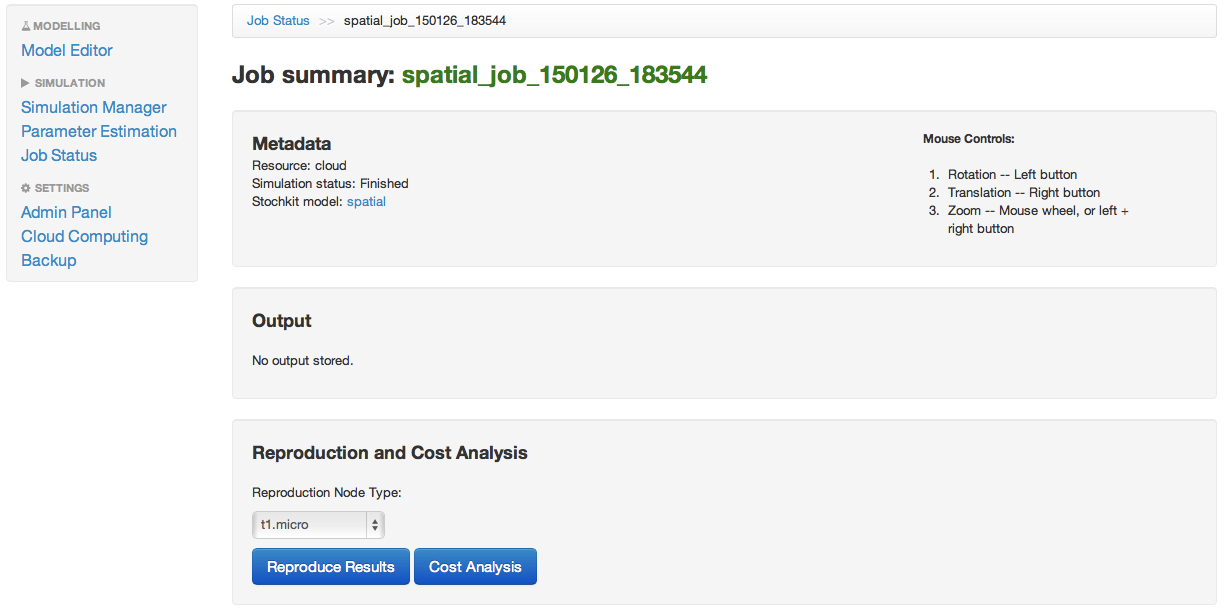
\includegraphics[scale=0.35]{T6/T6_fig_reproduction1.png}
\caption{Job summary page - reproduction available}
\label{fig:3}
\end{figure}

\section{Cost Analysis}
Because different instance types cost different amounts of money, it is not obvious which nodes are the cheapest for any given job type. StochSS allows manual measurement of job cost with the cost-analysis tool.

\subsection{An Example on Job Reproduction}

\begin{figure}[!ht]
\centering
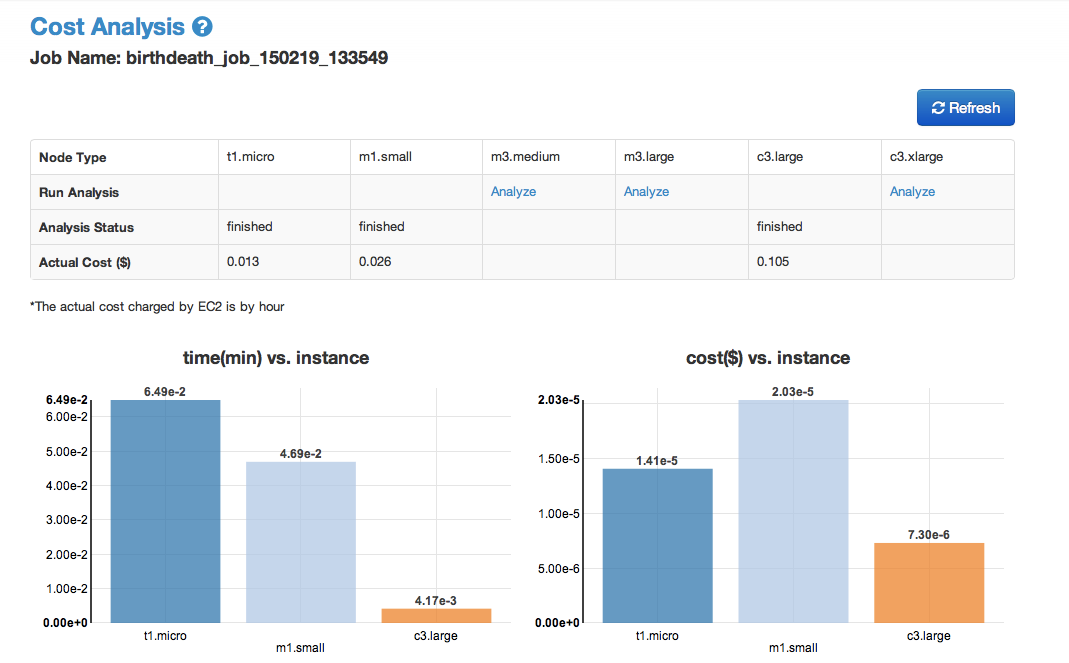
\includegraphics[scale=0.30]{T6/T6_fig_costanalysis.png}
\caption{Cost Analysis page}
\label{fig:cost-analysis}
\end{figure}

\begin{enumerate}
\item Run a well-mixed or spatial model.
\item Navigate to the \textbf{Job Status} page.
\item Click \textbf{view} beside the job you would like to analyze.
\item Click \textbf{Cost Analysis} in the \textbf{Reproduction and Cost Analysis} section.
\item By default, cost analysis should be available for whatever instance type the job was run on.
\item Click \textbf{Analyze} with any other node type you would like to run and analyze the job on. At least one node of this instance type must already be running.
\item The run times and costs of simulating the jobs are plotted on the screen as in Figure \ref{fig:cost-analysis}.
\end{enumerate}

%!TEX root = ../main.tex

\chapter{Parameter Sweeps}

It is often of interest to explore the parameter space of a model. We may want to find what the value of some parameters should be, or maybe we want to find regions in parameter space where the model exhibits interesting behavior.

StochSS supports sweeps over one or two parameters. To set up a parameter sweep, simply click \textbf{Parameter Sweep}. Select the model that you want to analyze, the parameters you want to analyze, the upper and lower bound of the parameters, and the number of steps in each parameter.

First import the \emph{lotkavolterra\_concentration\_oscil} model from the \emph{Public Library}. Select this model in the parameter sweep main window, and run a two-parameter sweep over $k1$ and $k2$. Click \textbf{Run Local}, and wait for the computation to finish. Once it has finished, the output can be visualized on the \textbf{Job Summary} page, see Figure \ref{psweep-fig1}. You have to select a \emph{mapper} and a \emph{reducer}, and can view the average concentrations, the max- and min-values, as well as the variance. As an example, if the \emph{mapper} is `final time', and the reducer is `average', then that means that you will plot the average of the populations at the final time point.
\begin{figure}[!ht]
\centering
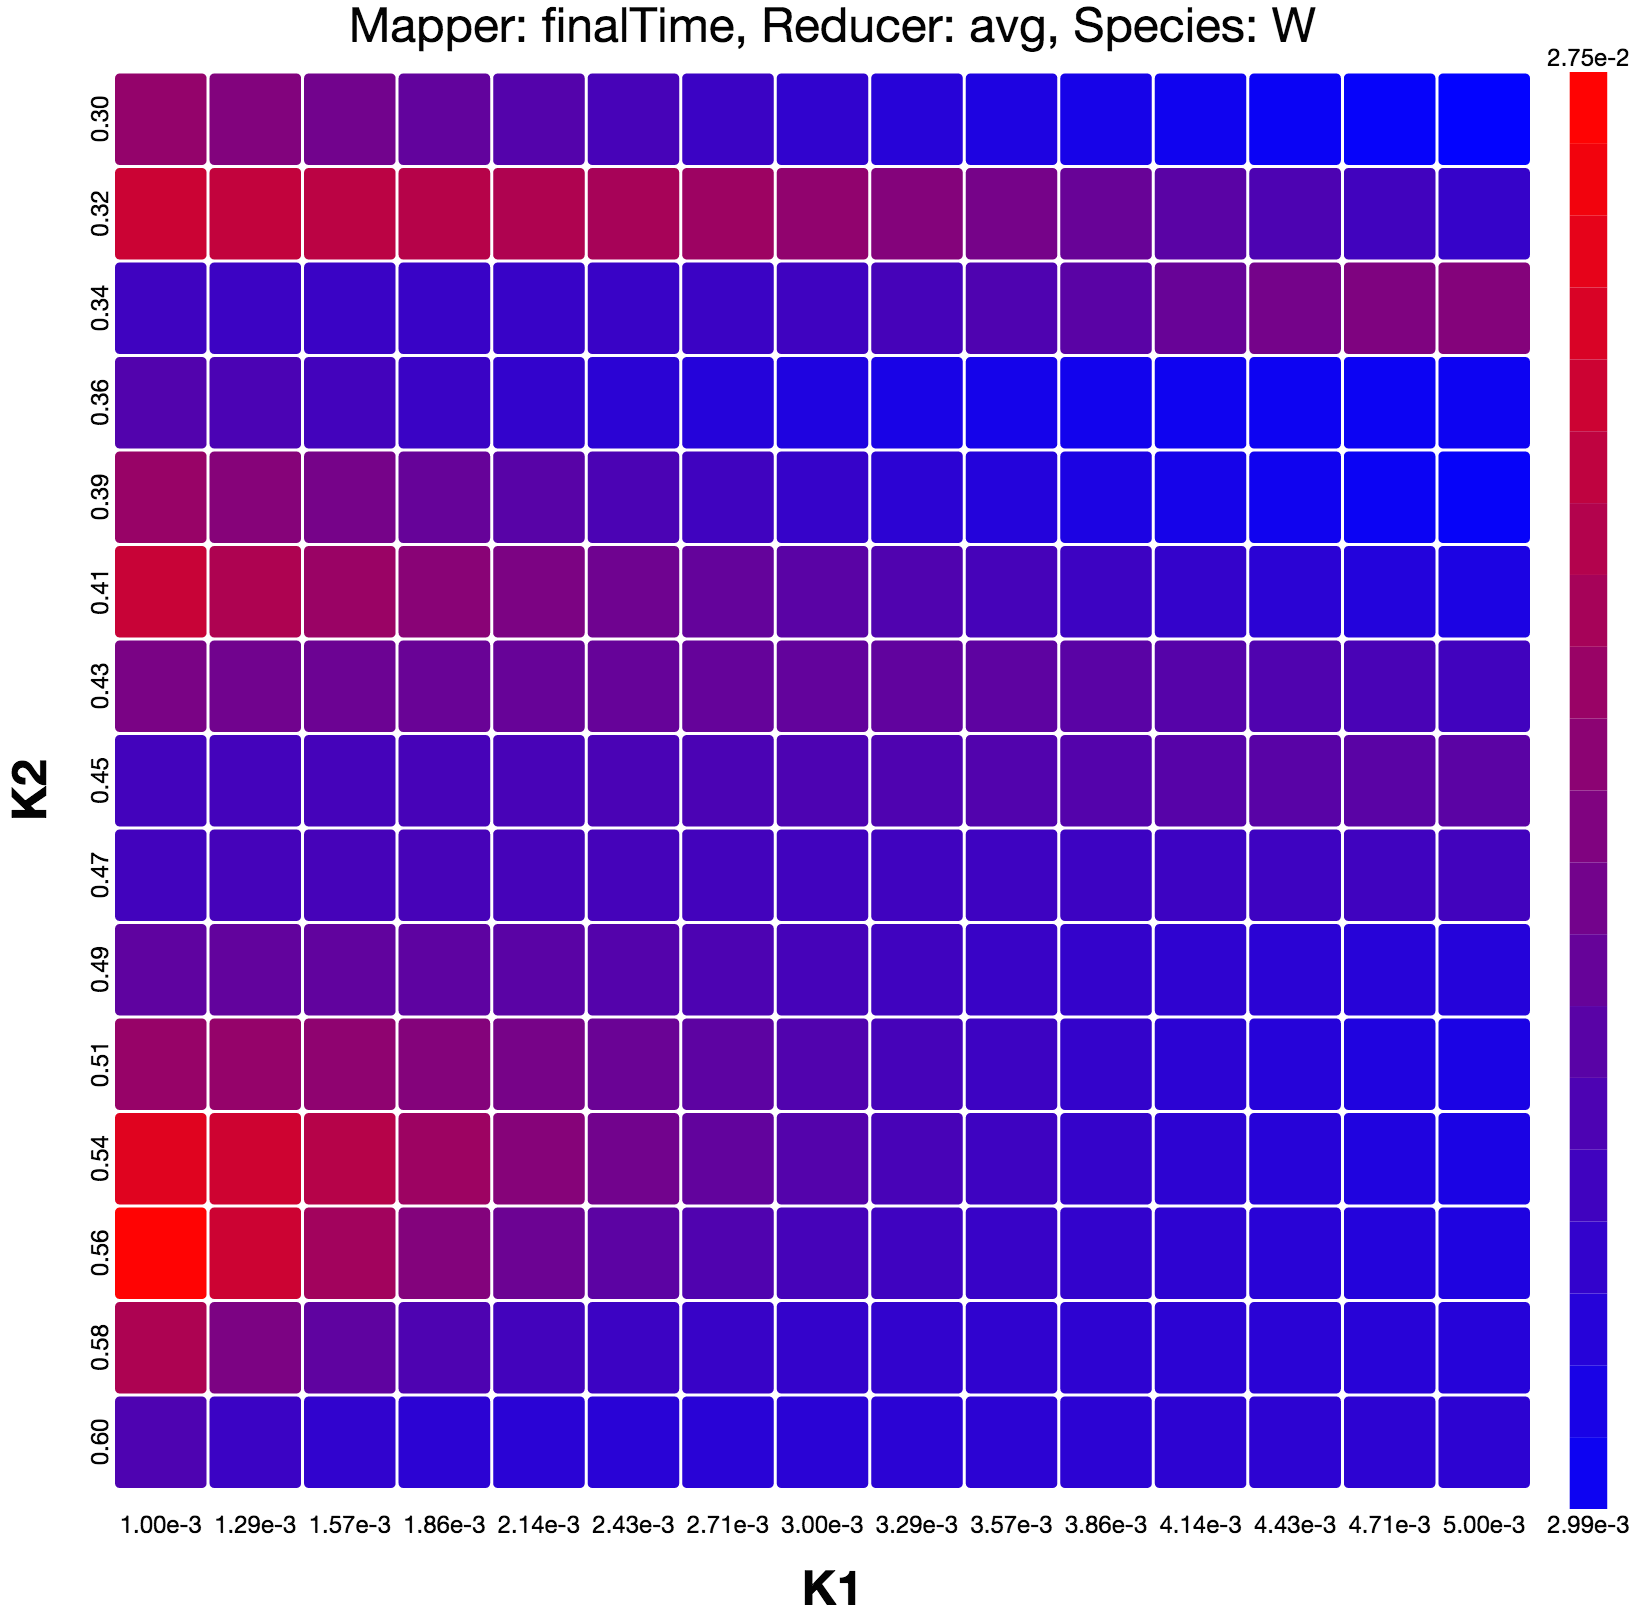
\includegraphics[width=0.95\textwidth]{Psweep/heatmap.png}
\caption{\label{psweep-fig1}A two-parameter sweep is visualized as a heat map. We have performed a sweep over the two parameters $k1$ and $k2$ of the \emph{lotkavolterra\_concentration\_oscil} model. }
\end{figure}

Finally, if you need to perform an in-depth analysis of the data, there is the option of exporting the parameter sweep to a Jupyter Notebook. On the \textbf{Job Summary} page, click \textbf{Analyze using interactive Jupyter Notebook}. This launches a Jupyter Notebook, with a template for analyzing the data. We recommend users unfamiliar with Jupyter to visit http://jupyter.org for full documentation and tutorials.


%!TEX root = ../main.tex

\chapter{Visualization}
Full three dimensional spatial stochastic simulations can be difficult to analyze. To simplify the process, StochSS has built in three different methods for visualization of spatial models.

\section{Surface Renderings with Domain Clipping}

By default, spatial stochastic simulations are rendered as shown in Figure \ref{surface}. These are surface renderings, but the simulations are volumetric. To see inside the volume, StochSS allows slicing the mesh in half along one axis with a plane and only rendering one of the resultant halves. This is shown in Figure \ref{clipx}

\begin{figure}[!ht]
  \centering
    \includegraphics[width=0.5\textwidth]{Vis/surface}
  \caption{ Surface rendering of cylindrical domain. The actual stochastic simulation is run on the dual of the shown mesh, so the color at each node corresponds to the concentration in the corresponding voxel of the dual mesh. Colors are interpolated linearly between nodes. The color scale is not shown for brevity. }
  \label{surface}
\end{figure}

\begin{figure}[!ht]
  \centering
    \includegraphics[width=0.5\textwidth]{Vis/clipx}
  \caption{ Surface rendering of cylindrical domain clipping along the X dimension. It is now possible to see concentrations of voxels inside the cylinder. }
  \label{clipx}
\end{figure}

\section{Colorized Wireframe Meshes}

The second rendering type is similar to the first, but instead of rendering surfaces only edges are rendered (see Figure \ref{wireframe}). The colorization is the same, it is just ideally easier to see inside the mesh. Similarly to the surface rendering the wireframe renderings can be clipped to get a clearer view of what is happening inside the volume. See Figure \ref{clipy} for a demonstration of clipping a mesh in the Y dimension.

\begin{figure}[!ht]
  \centering
    \includegraphics[width=0.5\textwidth]{Vis/wireframe}
  \caption{ Wireframe rendering of cylindrical domain. The colors are handled similarly to in Figure \ref{surface}. }
  \label{wireframe}
\end{figure}

\begin{figure}[!ht]
  \centering
    \includegraphics[width=0.5\textwidth]{Vis/clipy}
  \caption{ Wireframe rendering of cylindrical domain clipped in the Y direction. }
  \label{clipy}
\end{figure}

\section{Volume Rendering}

The final rendering StochSS offers is a volume rendering (Figure \ref{volume}). It uses a basic ray-tracing implementation following the one in \cite{congote}.

\begin{figure}[!ht]
  \centering
    \includegraphics[width=0.5\textwidth]{Vis/volume}
  \caption{ This is the volume rendering of the same data shown above. The idea behind volume rendering is to color darkly areas with high concentrations and leave volumes with low concentrations transparent. The transparency makes it possible to see inside a volume rendering, and so the slicing as shown in the surface and wireframe renderings is not used. }
  \label{ volume }
\end{figure}

\section{Visualization in Interactive Jupyter Notebook}

In many projects the need to perform custom postprocessing and visualization will eventually arise. To facilitate this process, StochSS offers the possibility to export a Jupyter Notebook template, which reads the output and plots the average populations of the species. The user can then customize the Notebook to perform the required postprocessing and plotting.

To access this function, simply click \textbf{Analyze using Interactive Notebook} on the \textbf{Job Summary} page. Figure \ref{vis-jupyter} shows the default template.

For documentation and tutorials on Jupyter Notebooks, see http://jupyter.org.

\begin{figure}[!ht]
\centering
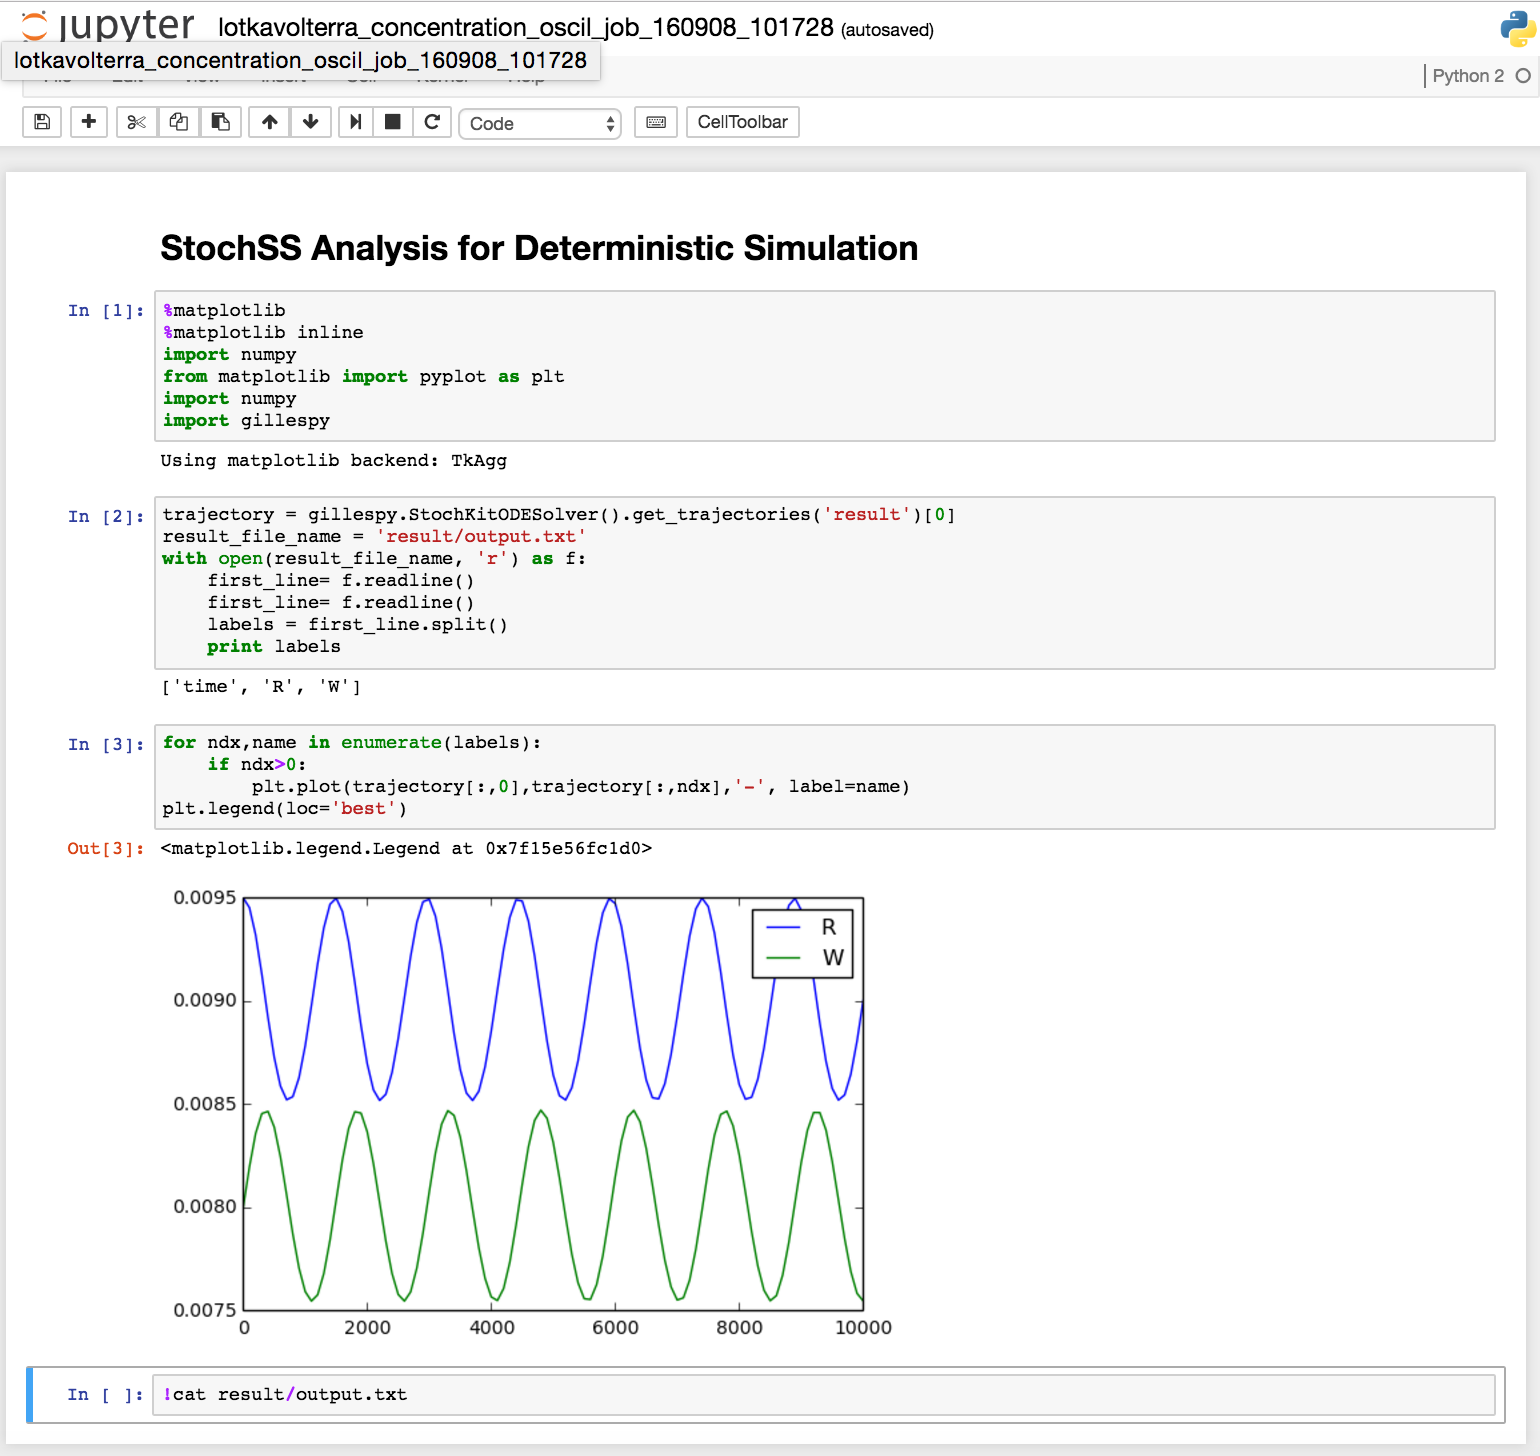
\includegraphics[width=0.8\textwidth]{Vis/vis-jupyter.png}
\caption{\label{vis-jupyter}Default Notebook for custom postprocessing.}
\end{figure}





\chapter{Flex Cloud}


StochSS 1.6 introduces Flex Cloud, an abstraction which allows you to run StochSS jobs on any machine, physical or virtual, provided it is running Ubuntu 12.04 with the required software dependencies installed. %Flex Cloud is a feature that should only be used by people familiar with the Linux operating systems, as it requires some detailed systems knowledge to set up.

\section{Setting Up Flex Cloud Compute Machines}

\subsection{Preparing the Flex Cloud compute nodes}
\begin{itemize}
\item Configure one or more machines running Ubuntu 12.04 (Precise). %It is recommended that these computers be dedicated solely to Flex Cloud, as to reduce the chance of interference between StochSS and other programs.
\item Please make sure the machines have their own IP address and are accessible with just a username and a passwordless SSH keypair. If necessary, generate SSH keypairs for the machines. You will need to upload the SSH private key to the StochSS user interface to access the machines.
\item Configure the firewall on the machines to allow connections on the following ports: 22, 5672, 6379, 11211, 55672, 80, 443, 3306. These are used for various services used by StochSS. If the machines are instances running on a public or private cloud, you may need to enable the ports by modifying the associated cloud security group. 
\item Install the software prerequisites on the machines by using the command line utility \emph{make\_flex\_vms.py}  which can be found in the StochSS Github repository in the directory \emph{release-tools/flex-cloud}. You can either specify the username, IP address, and SSH keys of the machines in a machine config file (an example one is included in the same directory for reference) or you can specify the machines on the command line. The script \emph{make\_flex\_vms.py} will also verify that the necessary network ports are open and working. Please see \emph{make\_flex\_vms.py -h} for further information.
\end{itemize}

\subsection{Configuring the compute nodes in StochSS}

\begin{itemize}
\item Click \textbf{Cloud Computing} to navigate to the main \textbf{Cloud Computing} page.
\item You have the option of selecting \textbf{Amazon AWS Cloud} or \textbf{Flex Cloud}. Select \textbf{Flex Cloud}. It will redirect you to \textbf{Flex Cloud Credentials} page. 

(Note: You cannot set up both Amazon AWS Cloud or Flex Cloud at the same time. If one cloud computing infrastructure has been set up, the link for the other infrastructure will be disabled on this page.)

%\begin{figure}[!ht]
%\centering
%\includegraphics[scale=0.45]{T7/T7_fig_flex_cloud_credentials_page.png}
%\caption{Flex Cloud Credentials page}
%\label{fig:2}
%\end{figure}

\item Click \textbf{Choose Files} to upload the SSH private keys (see Figure \ref{fig:2}).

\begin{figure}[!ht]
\centering
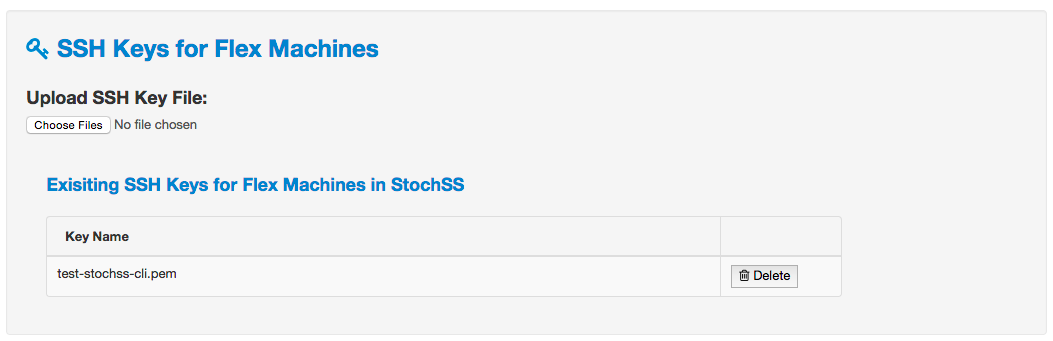
\includegraphics[scale=0.45]{T7/T7_fig_flex_uploaded_ssh_keys.png}
\caption{Uploaded SSH keys for Flex Machines -- Flex Cloud Credentials page}
\label{fig:2}
\end{figure}

\item Next, in the first row of the \textbf{Flex Cloud Machine Info} table, type the IP address and username, and select the appropriate key pair for the compute node that should act as the queue head. The Flex Queue Head will act as a coordinate for StochSS jobs, as well as store all output for jobs run in the cloud. This machine should be fairly robust; for EC2 instances a c3.large would be appropriate.
\item Click \textbf{+} to add more compute nodes. %For each of them, type the IP address, username, and enter the key info as above.
\item Click \textbf{Deploy} to start the Flex Cloud service.
\item The compute nodes may take a few minutes to launch. Refresh the page occasionally and wait until all nodes enter the \emph{running} state as shown in the \textbf{Flex Cloud Machine Info} table.

\item Once Flex Cloud has been successfully configured, StochSS will run jobs in Flex Cloud when you click \textbf{Run via Cloud} as long as Flex Cloud has been successfully configured and the Flex Queue Head node is up and running.

\item To stop Flex Cloud, click \textbf{Stop} on the Flex Cloud configuration page. (Note: \textbf{Stop} does not terminate/shut-down/reboot machines).

\warning{\newline Any data that is not downloaded from the Flex Cloud will be inaccessible while the Flex Cloud is turned off. Reconfiguring the queue head or keys without downloading job results can lead to data loss.\newline}

\end{itemize}


%!TEX root = main.tex

\chapter{Import a custom mesh}

When setting up a spatial problem in StochSS information about the geometry needs to be provided through two files: a
file containing the mesh information in DOLFIN XML format and a text file containing information about subdomains. The
file with subdomain information is optional in general (if it is not provided the entire mesh will belong to one subdomain).
Below is a tutorial on how to provide that information in a variety of cases.

\section{Mesh library}

The first and simplest scenario is using one of the default built-in meshes provided by StochSS in the Mesh Library.
These include simple example mesh and subdomain combinations that are common in biological modeling. For example
there is a unit sphere with a membrane (i.e. the volume is one subdomain and the surface is another), a unit cube witha
membrane, a cylinder with the two ends being different subdomains among others. If for a given problem these are not
sufficient then mesh and subdomain information can be provided by attaching files. One simple case where creating and
attaching a file may be necessary could involve using the DOLFIN built in meshes but with different subdomains than
provided in the Mesh Library. This can be done as follows.

\section{Using DOLFIN Built-In Geometry with Subdomains Outside of Mesh Library}

For example consider a sphere with three different subdomains: the top half of the membrane, the bottom half of the
membrane and the volume. This can be done using PyURDME as follows (PyURDME and FEniCS are software packages
that are automatically installed during the StochSS installation and DOLFIN is a library within FEniCS).

In an IPython Notebook, import the appropriate libraries:

\begin{ipythonnb}
import os,pyurdme,dolfin
\end{ipythonnb}

Next classes are constructed to define the desired subdomains:

\begin{ipythonnb}
class top_half_membrane(dolfin.SubDomain):
	def inside(self,x,on_boundary):
	return on_boundary and x[2]>=0
	
class bottom_half_membrane(dolfin.SubDomain):
	def inside(self,x,on_boundary):
	return on_boundary and x[2]<=0
\end{ipythonnb}

Then a pyurdme model is created with the desired geometry and marked subdomains:

\begin{ipythonnb}
class sphere_top_bot(pyurdme.URDMEModel):
	def __init__(self,model_name="polarization"):
		pyurdme.URDMEModel.__init__(self,model_name)
		
		#DefineGeometry
		sphere=dolfin.Sphere(dolfin.Point(0.0,0.0,0.0),1.0)
		self.mesh=pyurdme.URDMEMesh(mesh=dolfin.Mesh(sphere,10))

		cell_function=dolfin.CellFunction("size_t",self.mesh)
		cell_function.set_all(1)

		facet_function=dolfin.FacetFunction("size_t",self.mesh)
		facet_function.set_all(0)

		top_membrane=top_half_membrane()
		top_membrane.mark(facet_function,2)

		bottom_membrane=bottom_half_membrane()
		bottom_membrane.mark(facet_function,3)

		self.add_subdomain(cell_function)
		self.add_subdomain(facet_function)

		#Define initial populations
		self.set_initial_condition_scatter({},[1])
\end{ipythonnb}

\begin{ipythonnb}
model = sphere_top_bot()
\end{ipythonnb}

The subdmain infomation can then be extracted from the model as follows:
\begin{ipythonnb}
sd = model.get_subdomain_vector()
\end{ipythonnb}

And finally two files are created to store the mesh and subdomain information respectively in the the correct format:
\begin{ipythonnb}
\# This is a dolfin xml file with mesh information
dolfin.File("sphere_top_bot_mesh.xml") << model.mesh
\end{ipythonnb}

\begin{ipythonnb}
\ampersand This is the file to capture information about subdomains
with open("sphere_top_bot_subdomains.txt",'w') as fd:
	for ndx,val in enumerate(sd):
		fd.write("{0},{1}\n".format(ndx,val))
\end{ipythonnb}
Now that these two files have been created they can be attached in the Mesh tab of the model editor in StochSS and the
rest of the problem can be defined from there. Again it is important to note that if a problem does not involve subdomains
then only the mesh XML file is necessary and the entire mesh will be given the same domain! One last situation that could
arise in defining spatial information is that a mesh has to be created in external software then converted to the correct
format.

\section{Advanced mesh generation}

For many real world applications the geometry involved will be more complicated than the built?in meshes provided by
DOFLIN (and by extension StochSS). In these situations a mesh will have to be created in an external program such as
Gmsh then converted into the DOLFIN XML format. Once the mesh has been created in an external program the
conversion to DOLFIN XML format can easily be done by the built in script dolfin?convert [1]. The following command line
code demonstrates how to convert from the Gmsh format (suffix .msh or .gmsh) to DOLFIN XML format.

The following needs to be run from the command line in the Terminal:
\begin{verbatim}
dolfin-convert mesh.msh mesh.xml
\end{verbatim}

File formats that are currently supported by the dolfin-convert script can be found in the table below:

\begin{table}[htp]
   \begin{tabular}{| l | l |} % Column formatting, @{} suppresses leading/trailing space
   \toprule
      Suffix   & File Format\\
      \midrule
     .xml & DOLFIN XML format\\
     .ele / .node & Triangle file format\\
     .mesh & Medit format, generated by TetGen with option ?g\\
     .msh / .gmsh & Gmsh version 2.0 format\\
     .grid & Diffpack tetrahedral grid format\\
     .inp & Diffpack tetrahedral grid format\\
     .e / .exo & Sandia Exodus II file format\\
     .ncdf & ncdump'ed Exodus II file format\\
     .vrt / .cell & StarCD tetrahedral grid format\\
     \bottomrule
   \end{tabular}
   \end{table}



The XML file that is created from the dolfin?convert command can then be used directly in StochSS. If subdomains are
required then a text file can be created using code similar to that above. Consider the situation where the XML file created
was called "coli.xml" then the code to create a subdomain file consisting of the outer membrane would look as follows:

\begin{ipythonnb}
import os,pyurdme,dolfin
\end{ipythonnb}

\begin{ipythonnb}
class Membrane(dolfin.SubDomain):
	def inside(self,x,on_boundary):
	return on_boundary
\end{ipythonnb}

\begin{ipythonnb}
class ecoli(pyurdme.URDMEModel):
	def __init__(self,model_name="polarization"):
		pyurdme.URDMEModel.__init__(self,model_name)
		
		\#DefineGeometry
		self.mesh=pyurdme.URDMEMesh(mesh=dolfin.Mesh('coli.xml'))

		cell_function=dolfin.CellFunction("size_t",self.mesh)
		cell_function.set_all(1)

		facet_function=dolfin.FacetFunction("size_t",self.mesh)
		facet_function.set_all(0)

		membrane=Membrane()
		membrane.mark(facet_function,2)

		self.add_subdomain(cell_function)
		self.add_subdomain(facet_function)

		\#Define initial populations
		self.set_initial_condition_scatter({},[1])
\end{ipythonnb}

\begin{ipythonnb}
model=ecoli()
\end{ipythonnb}

\begin{ipythonnb}
sd=model.get_subdomain_vector()
\end{ipythonnb}

\begin{ipythonnb}
\#This is the file to capture information about subdomains
with open("coli_subdomains.txt",'w') as fd:
	for ndx,val in enumerate(sd):
		fd.write("{0},{1}\n".format(ndx,val))
\end{ipythonnb}

Now all of the necessary files have been created. The "coli.xml" file that was created using a dolfin?convert command and
the "coli\_subdomains.txt" just created can be uploaded directly to StochSS and used accordingly.

\section{References}

1. A. Logg, K.?A. Mardal, G. N. Wells et al. Automated Solution of Partial Differential Equations by the Finite Element Method: The FEniCS Book. Springer 2012.





\begin{thebibliography}{9}

\bibitem{dan}
  D.T. Gillespie.
  \textit{Exact stochastic simulation of coupled chemical reactions}.
  J. Phys. Chem., 81(25), 2340-2361 (1977)

\bibitem{sundials}
  A. C. Hindmarsh et al.,
  \textit{SUNDIALS: Suite of nonlinear and differential/algebraic equation solvers}.
  ACM Trans. Math. Softw., 31(3), 363-396 (2005)
  
  \bibitem{scale}
  W. A. Link and P. F. Doherty Jr.,
  \textit{Scaling in sensitivity analysis}.
  Ecology, 83(12), 3299-3305 (2002)
  
  \bibitem{calib}
  M. C. Hill,
  \textit{Methods and guidelines for effective model calibration}. 
  U.S. Geol. Surv. Water Resour. Invest. Rep. 98-4005 (1998)
  
  \bibitem{bernie}
  B.J. Daigle et al.
  \textit{Accelerated maximum likelihood parameter estimation for stochastic biochemical systems}.
  BMC Bioinformatics, 13, 68 (2012)
  
  \bibitem{caffo}
  B.S. Caffo et al.
  \textit{Ascent-based Monte Carlo expectation-maximization}. 
  J. Royal Statistical Society Series B, 67(2), 235-251 (2005)
  
  \bibitem{nsm}
  J. Elf and M. Ehrenberg,
  \textit{Spontaneous separation of bi-stable biochemical systems into spatial domains of opposite phases}. IEEE Systems Biology, 1, 230-6 (2004)
  
 \bibitem{urdme}
 B. Drawert, S. Engblom and A. Hellander, 
 \textit{URDME: {A} modular framework for stochastic simulation
of reaction-transport processes in complex geometries}. BMC Systems Biology, 6(76) (2012)
  
  \bibitem{wiki-michaelis-menten}
  Michaelis-Menten kinetics. 
  \url{http://en.wikipedia.org/wiki/Michaelis-Menten_kinetics}
  
  \bibitem{congote}
  Congote, John and Segura, Alvaro and Kabongo, Luis and Moreno, Aitor and Posada, Jorge and Ruiz, Oscar.
  \textit{Interactive Visualization of Volumetric Data with WebGL in Real-time}
  In Proceedings of the 16th International Conference on 3D Web Technology (Web3D '11). ACM, New York, NY, USA, 137-146.
  \url{http://dx.doi.org/10.1145/2010425.2010449}
  
\end{thebibliography}


\end{document}
